\begin{figure}[t!]
    \centering
    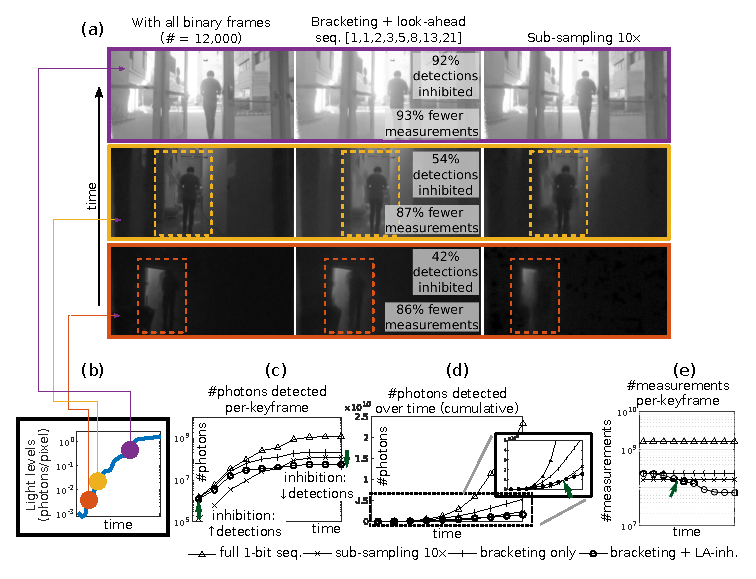
\includegraphics[width=\textwidth]{figures/qbp_swissSPAD2/qbp_long_hdr_seq}
    \caption{\textbf{Adaptive policies on video sequences enable stronger inhibition, preserve low-light details and, in bright-light, decouple flux and detection energy.}
    (a) Burst reconstructions \cite{maQuantaBurstPhotography2020a} for three keyframes with varying light levels: the top and bottom row differ by $\approx$ 7 stops.
    [Images show the detection rates $Y$ and are further gamma-compressed ($\gamma = 0.4$).
    Complete results included in the supplement.]
    Left column results are from the original binary frames without inhibition, and the right column after sub-sampling $10\times$ (a fixed $90\%$ inhibition). Middle column represents exposure bracketing combined with saturation look-ahead (see Fig.~\ref{table:sat_lookahead_policy}a for description).
    Under strong light (top row) the results are reasonable with both methods.
    However, plain sub-sampling loses details in lower light: notice the furniture and a person's outline in the middle \& bottom rows, respectively.
    Inhibition is instead adaptive to flux.  
    (b) Average exposure level for each keyframe in the sequence.
    (c,d) Per-keyframe and cumulative detection counts -- inhibition ultimately results in fewer photons being detected over the whole sequence. (e) Number of measurements taken for each keyframe; reductions may be translated to energy savings during read-out. Plots in (c,d,e) are sub-sampled for clarity, and crossover points are marked by green arrows.
    }
    \label{fig:qbp_long_hdr_seq}
\end{figure}
